% Options for packages loaded elsewhere
\PassOptionsToPackage{unicode}{hyperref}
\PassOptionsToPackage{hyphens}{url}
%
\documentclass[
]{book}
\usepackage{lmodern}
\usepackage{amssymb,amsmath}
\usepackage{ifxetex,ifluatex}
\ifnum 0\ifxetex 1\fi\ifluatex 1\fi=0 % if pdftex
  \usepackage[T1]{fontenc}
  \usepackage[utf8]{inputenc}
  \usepackage{textcomp} % provide euro and other symbols
\else % if luatex or xetex
  \usepackage{unicode-math}
  \defaultfontfeatures{Scale=MatchLowercase}
  \defaultfontfeatures[\rmfamily]{Ligatures=TeX,Scale=1}
\fi
% Use upquote if available, for straight quotes in verbatim environments
\IfFileExists{upquote.sty}{\usepackage{upquote}}{}
\IfFileExists{microtype.sty}{% use microtype if available
  \usepackage[]{microtype}
  \UseMicrotypeSet[protrusion]{basicmath} % disable protrusion for tt fonts
}{}
\makeatletter
\@ifundefined{KOMAClassName}{% if non-KOMA class
  \IfFileExists{parskip.sty}{%
    \usepackage{parskip}
  }{% else
    \setlength{\parindent}{0pt}
    \setlength{\parskip}{6pt plus 2pt minus 1pt}}
}{% if KOMA class
  \KOMAoptions{parskip=half}}
\makeatother
\usepackage{xcolor}
\IfFileExists{xurl.sty}{\usepackage{xurl}}{} % add URL line breaks if available
\IfFileExists{bookmark.sty}{\usepackage{bookmark}}{\usepackage{hyperref}}
\hypersetup{
  pdftitle={Estadísticas Oficiales Institucionales},
  pdfauthor={Alberto Rodríguez Rodríguez},
  hidelinks,
  pdfcreator={LaTeX via pandoc}}
\urlstyle{same} % disable monospaced font for URLs
\usepackage{longtable,booktabs}
% Correct order of tables after \paragraph or \subparagraph
\usepackage{etoolbox}
\makeatletter
\patchcmd\longtable{\par}{\if@noskipsec\mbox{}\fi\par}{}{}
\makeatother
% Allow footnotes in longtable head/foot
\IfFileExists{footnotehyper.sty}{\usepackage{footnotehyper}}{\usepackage{footnote}}
\makesavenoteenv{longtable}
\usepackage{graphicx}
\makeatletter
\def\maxwidth{\ifdim\Gin@nat@width>\linewidth\linewidth\else\Gin@nat@width\fi}
\def\maxheight{\ifdim\Gin@nat@height>\textheight\textheight\else\Gin@nat@height\fi}
\makeatother
% Scale images if necessary, so that they will not overflow the page
% margins by default, and it is still possible to overwrite the defaults
% using explicit options in \includegraphics[width, height, ...]{}
\setkeys{Gin}{width=\maxwidth,height=\maxheight,keepaspectratio}
% Set default figure placement to htbp
\makeatletter
\def\fps@figure{htbp}
\makeatother
\setlength{\emergencystretch}{3em} % prevent overfull lines
\providecommand{\tightlist}{%
  \setlength{\itemsep}{0pt}\setlength{\parskip}{0pt}}
\setcounter{secnumdepth}{5}
\usepackage{booktabs}
\usepackage[]{natbib}
\bibliographystyle{apalike}

\title{Estadísticas Oficiales Institucionales}
\usepackage{etoolbox}
\makeatletter
\providecommand{\subtitle}[1]{% add subtitle to \maketitle
  \apptocmd{\@title}{\par {\large #1 \par}}{}{}
}
\makeatother
\subtitle{Guía Metodológica}
\author{Alberto Rodríguez Rodríguez}
\date{2021-01-20}

\begin{document}
\maketitle

{
\setcounter{tocdepth}{1}
\tableofcontents
}
\hypertarget{portada}{%
\chapter*{Portada}\label{portada}}
\addcontentsline{toc}{chapter}{Portada}

\begin{center}
\includegraphics[width=0.75\linewidth]{imagenes/Portada} \end{center}

\hypertarget{intro}{%
\chapter{\texorpdfstring{\textbf{Introducción}}{Introducción}}\label{intro}}

\hypertarget{quuxe9-y-cuxf3mo-medir}{%
\chapter{\texorpdfstring{\textbf{¿Qué y cómo medir?}}{¿Qué y cómo medir?}}\label{quuxe9-y-cuxf3mo-medir}}

Las posibilidades existentes y alcanzables a través de la gestión de los datos en las universidades son tan numerosas que es fundamental priorizar y establecer una gestión que maximice las necesidades cuantitativas institucionales y del país a un costo financiero, humano, administrativo, académico y técnico razonable. Para ello se propone un enfoque minimalista. El minimalismo, en términos generales, hace referencia a la tendencia de volver a lo esencial, reducir una expresión a lo básico, eliminando aspectos sobrantes o accesorios. Esta es una corriente que inicia en el ámbito artístico y ha sido adoptada para diferentes usos, como obras de arte y decoración de ambientes. En este documento proponemos enfrentar, en un primer paso, la sobreinformación con minimalismo para una gestión de la información más efectiva a sus propósitos.

Es posible y deseable adelantar apuestas de \emph{Big Data} en las universidades, así como apuestas de minería o analítica de datos y estudios cuantitativos con propósitos causales o evaluaciones profundas a políticas institucionales, aunque académica, metodológica, operativa y financieramente resulta costoso. Cada vez existen más lineamientos y presiones a nivel estatal para ir en esta dirección, sin embargo, lo que actualmente más se le demanda a las universidades en Colombia es la carga de microdatos para sistemas de información externos, y la construcción y disposición de cifras estadísticas e indicadores institucionales.

Haciendo uso de los diferentes niveles que acompañan actualmente la gestión de la información cuantitativa en las universidades\footnote{Los niveles se expusieron de manera detallada en el capítulo anterior y se ilustraron en la figura \ref{fig:fig15}.}, la tabla 2 presenta el resultado de priorización --apuesta minimalista-- que ha emprendido la Universidad Nacional de Colombia para enfrentar el contexto actual de demanda de información cuantitativa que se experimenta a nivel interno, el cual hace uso del acercamiento más simple a los datos --descriptivo--, responde a la mayoría de las exigencias internas y externas en materia de gestión y disposición de las cifras institucionales, y aprovecha aquellas herramientas tecnológicas de alta calidad y accesibles para cualquier universidad pública dados sus bajos costos.

\textbf{Tabla 2.} \emph{Actividades priorizadas en materia de gestión estadística en la Universidad Nacional de Colombia}

\begin{longtable}[]{@{}lcc@{}}
\toprule
\begin{minipage}[b]{0.04\columnwidth}\raggedright
\strut
\end{minipage} & \begin{minipage}[b]{0.18\columnwidth}\centering
\textbf{Preguntas orientadoras}\strut
\end{minipage} & \begin{minipage}[b]{0.69\columnwidth}\centering
\textbf{Respuesta. Prioridad en la Universidad Nacional de Colombia -- Apuesta minimalista}\strut
\end{minipage}\tabularnewline
\midrule
\endhead
\begin{minipage}[t]{0.04\columnwidth}\raggedright
\textbf{Contexto de las cifras en la universidad estatal colombiana}\strut
\end{minipage} & \begin{minipage}[t]{0.18\columnwidth}\centering
\textbf{Nivel 1.1} ¿Por qué y para qué son útiles las cifras cuantitativas en el escenario de la universidad estatal contemporánea?\strut
\end{minipage} & \begin{minipage}[t]{0.69\columnwidth}\centering
Gestionar y disponer el legado histórico y numérico de esta universidad, contar con más y mejor información para la planeación y la toma de decisiones institucionales, mejorar los niveles de monitoreo y seguimiento a políticas institucionales y aumentar los niveles de transparencia institucional a través de un ejercicio de rendición cuantitativa de cuentas de manera permanente.\strut
\end{minipage}\tabularnewline
\begin{minipage}[t]{0.04\columnwidth}\raggedright
\strut
\end{minipage} & \begin{minipage}[t]{0.18\columnwidth}\centering
\textbf{Nivel 1.2} ¿Qué normas o lineamientos existen a nivel nacional e internacional para orientar la construcción y disposición de cifras en el contexto de las entidades públicas y, en especial, en las universidades? y ¿cuál es el alcance a nivel institucional de dichas normas y lineamientos?\strut
\end{minipage} & \begin{minipage}[t]{0.69\columnwidth}\centering
Conocer y aplicar, en el contexto de las posibilidades, los lineamientos expedidos en materia de gestión de información cuantitativa por parte de entidades nacionales como: \textbf{Sector de la educación y CTI:} MEN (CESU-CNA, Conaces, SNIES, Spadies, OLE), Colciencias y OCyT. DANE: Plan Estadístico Nacional y NTCPE 1000. DNP: \emph{Guía metodológica para el seguimiento y la evaluación a políticas públicas.} DAFP: MIPG, \emph{Manual Único de rendición de cuentas}, guía(s) para la construcción de indicadores. MinTIC: Gobierno Digital, datos abiertos. Secretaría de la Transparencia: Ley de transparencia. Contraloría: MECI, Sireci. Contexto internacional: ONU, OCDE, Unesco, Eurostat, Cepal, Manuales internacionales (Frascati, Oslo).\strut
\end{minipage}\tabularnewline
\begin{minipage}[t]{0.04\columnwidth}\raggedright
\strut
\end{minipage} & \begin{minipage}[t]{0.18\columnwidth}\centering
\textbf{Nivel 1.3} ¿Cuál es el uso y alcance que se dará a los datos disponibles a nivel institucional?\strut
\end{minipage} & \begin{minipage}[t]{0.69\columnwidth}\centering
Disponer de las cifras y los indicadores que se le demandan a la Universidad. Las principales demandas internas y externas que vive la universidad pública actual en Colombia y como consecuencia, las que más se gestionan en su interior son: estadísticas oficiales, indicadores de gestión, indicadores de desempeño, indicadores de eficiencia, indicadores de eficacia, indicadores de efectividad, indicadores de rentabilidad pública, indicadores de procesos, indicadores de proyectos, indicadores de planes de desarrollo, indicadores de calidad, indicadores de productos, indicadores de resultados, indicadores de impacto, indicadores ambientales, indicadores de economía, datos públicos, datos abiertos, cifras agregadas de aspirantes, estudiantes admitidos, estudiantes matriculados, graduados, docentes, funcionarios administrativos, investigadores, grupos de investigación, productos de investigación (publicaciones, patentes, citaciones, etc.), programas académicos, movilidad entrante y saliente a nivel nacional e internacional de docentes y estudiantes, cobertura en programas de bienestar universitario y capacidad financiera.\strut
\end{minipage}\tabularnewline
\begin{minipage}[t]{0.04\columnwidth}\raggedright
\strut
\end{minipage} & \begin{minipage}[t]{0.18\columnwidth}\centering
\textbf{Nivel 1.4} ¿Qué modelo o cuáles modelos organizacionales orientarán la gestión de los datos disponibles?\strut
\end{minipage} & \begin{minipage}[t]{0.69\columnwidth}\centering
Responder a las necesidades derivadas de la gestión por procesos, la gestión funcional y la gestión por proyectos existentes en la Universidad.\strut
\end{minipage}\tabularnewline
\begin{minipage}[t]{0.04\columnwidth}\raggedright
\textbf{Contexto académico y técnico de los datos}\strut
\end{minipage} & \begin{minipage}[t]{0.18\columnwidth}\centering
\textbf{Nivel 2.1} ¿Qué tipos de datos existen a nivel institucional y cuáles vamos a gestionar?\strut
\end{minipage} & \begin{minipage}[t]{0.69\columnwidth}\centering
Aprovechar la existencia y disposición de datos de tipo estructurado.\strut
\end{minipage}\tabularnewline
\begin{minipage}[t]{0.04\columnwidth}\raggedright
\strut
\end{minipage} & \begin{minipage}[t]{0.18\columnwidth}\centering
\textbf{Nivel 2.2} ¿Bajo qué disciplina o tendencia serán analizados los datos?\strut
\end{minipage} & \begin{minipage}[t]{0.69\columnwidth}\centering
Utilizar recursos heredados de la estadística y la inteligencia de negocios.\strut
\end{minipage}\tabularnewline
\begin{minipage}[t]{0.04\columnwidth}\raggedright
\strut
\end{minipage} & \begin{minipage}[t]{0.18\columnwidth}\centering
\textbf{Nivel 2.3} ¿Qué queremos responder y qué uso, en términos de análisis, haremos de los datos disponibles a nivel institucional?\strut
\end{minipage} & \begin{minipage}[t]{0.69\columnwidth}\centering
Aproximarnos de manera descriptiva a los datos estructurados disponibles.\strut
\end{minipage}\tabularnewline
\begin{minipage}[t]{0.04\columnwidth}\raggedright
\strut
\end{minipage} & \begin{minipage}[t]{0.18\columnwidth}\centering
\textbf{Nivel 2.4} ¿Qué método o técnica emplearemos para dar respuesta a las preguntas de interés institucional?\strut
\end{minipage} & \begin{minipage}[t]{0.69\columnwidth}\centering
Hacer uso de conteos, proporciones, visualización, razones, índices, tasas, distribuciones.\strut
\end{minipage}\tabularnewline
\begin{minipage}[t]{0.04\columnwidth}\raggedright
\strut
\end{minipage} & \begin{minipage}[t]{0.18\columnwidth}\centering
\textbf{Nivel 2.5} ¿Cuáles fundamentos o bases teóricas soportan los métodos o las técnicas cuantitativas empleadas a nivel institucional?\strut
\end{minipage} & \begin{minipage}[t]{0.69\columnwidth}\centering
Construcción y disposición, a partir de información poblacional, de estadísticas, indicadores, KPI, teniendo como base las enseñanzas de la aritmética.\strut
\end{minipage}\tabularnewline
\begin{minipage}[t]{0.04\columnwidth}\raggedright
\strut
\end{minipage} & \begin{minipage}[t]{0.18\columnwidth}\centering
\textbf{Nivel 2.6} ¿Cuáles herramientas tecnológicas se requieren para la gestión de los datos disponibles a nivel institucional?\strut
\end{minipage} & \begin{minipage}[t]{0.69\columnwidth}\centering
Hacer uso de herramientas tecnológicas como Excel, R, HTLM, JavaScript, CSS y disponer la información a través de \emph{dashboards}, presentaciones web, libros web y boletines digitales.\strut
\end{minipage}\tabularnewline
\bottomrule
\end{longtable}

El ejercicio de priorización que ha emprendido la Universidad Nacional en el contexto de la gestión de los datos institucionales disponibles a nivel administrativo, que se sintetiza en la figura \ref{fig:fig16}, es una de las probables rutas que pudiera haberse emprendido en materia de gestión estadística. No obstante, esta aproximación da respuesta a la mayoría de las necesidades internas y externas que experimenta esta institución en la actualidad a unos costos institucionales razonables.

\begin{figure}

{\centering 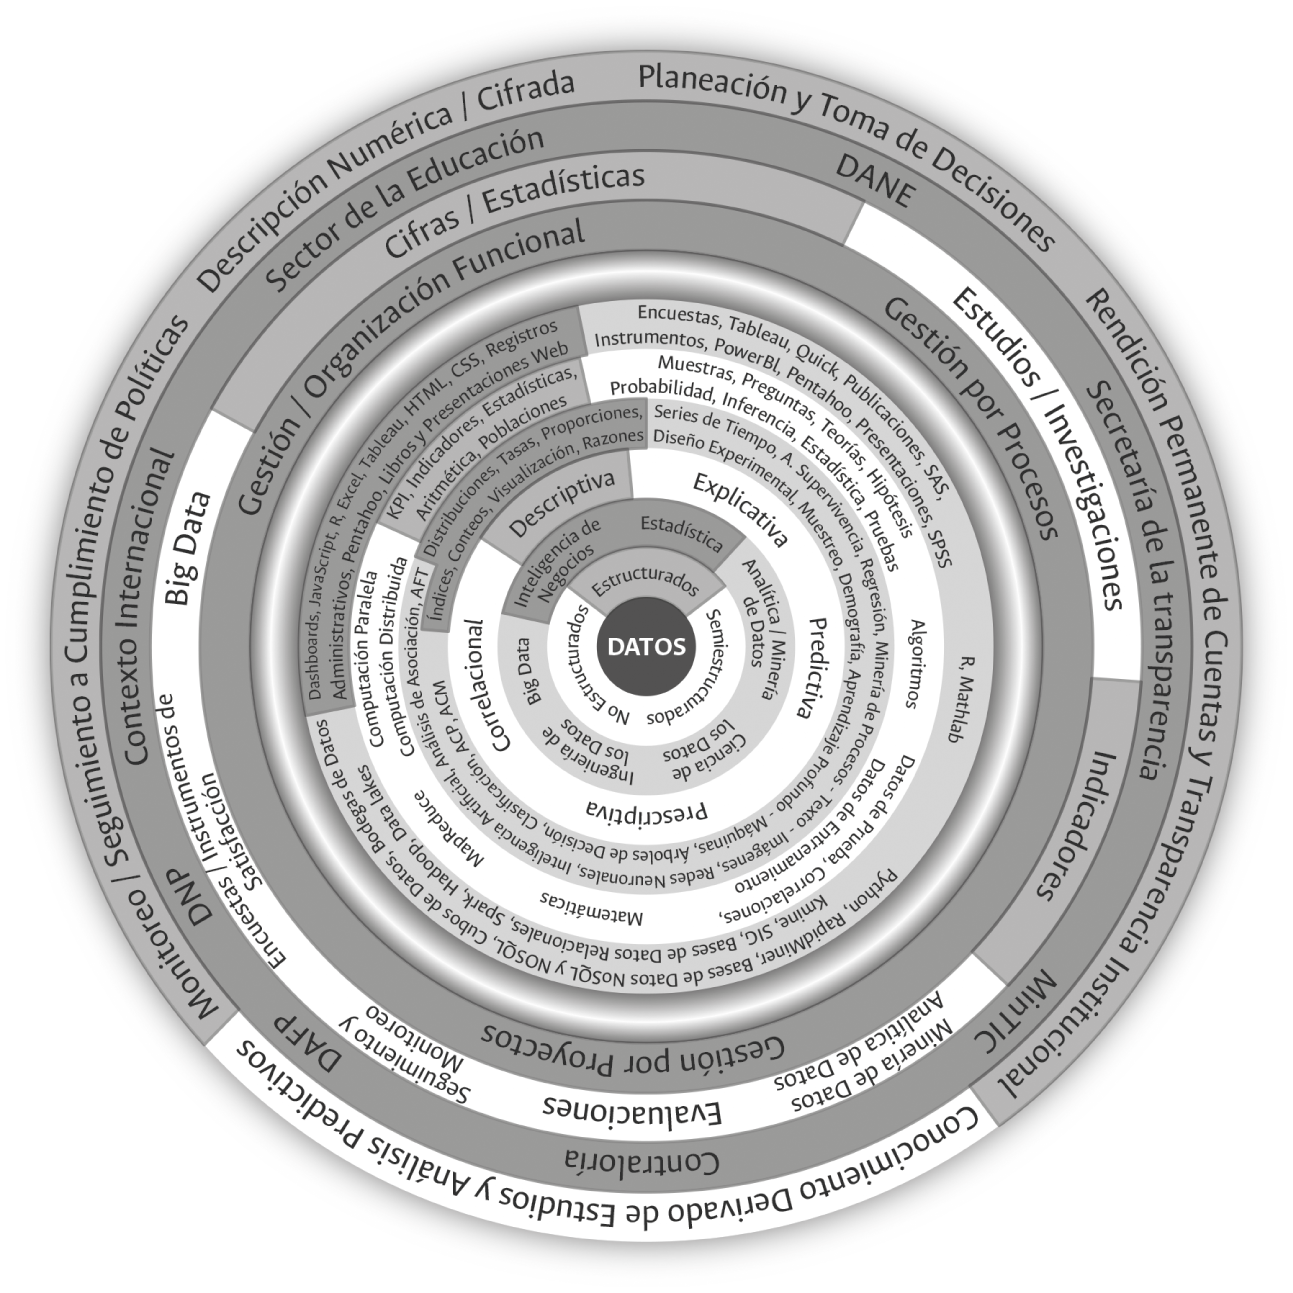
\includegraphics[width=0.75\linewidth]{imagenes/F_16} 

}

\caption{Alcance de la gestión estadística actual en la Universidad Nacional de Colombia en el contexto contemporáneo de los datos. Fuente: elaboración propia.}\label{fig:fig16}
\end{figure}

En el contexto contemporáneo de los datos cuantitativos son de gran utilidad tanto las aproximaciones descriptivas como aquellas que hacen uso de técnicas e instrumentos sofisticados; sin embargo, la cultura estadística en las entidades que conforman el Estado será difícil de alcanzar si se inicia con la aplicación del procedimiento más complejo; no se escala una montaña iniciando por su cima. La cultura estadística en la Universidad Nacional de Colombia y en otras universidades y entidades es posible de alcanzar si se inicia por lo esencial y, de manera reflexiva, se avanza hacia lo complejo.

\hypertarget{diferencia-entre-estaduxedsticas-e-indicadores}{%
\section{\texorpdfstring{\textbf{Diferencia entre estadísticas e indicadores}}{Diferencia entre estadísticas e indicadores}}\label{diferencia-entre-estaduxedsticas-e-indicadores}}

La aproximación descriptiva de los datos disponibles en las universidades públicas, en la que nos concentraremos en lo que resta del presenta capítulo, está atravesada por dos acepciones de uso frecuente tanto en la cotidianidad de la gestión estadística a nivel de las universidades como en la normatividad y los lineamientos metodológicos expedidos por entidades nacionales e internacionales en lo referente a la materia: las cifras estadísticas (o estadísticas) y los indicadores. Hoy el lenguaje dominante en el escenario de lo público es el de los indicadores; no obstante, ayer era el de las estadísticas. No nos concentraremos en los antecedentes históricos sobre el origen y posicionamiento de estas acepciones y sobre las diferentes tipologías que las acompañan. Consideramos pertinente, por el momento, hacer una separación entre estos dos términos y, en especial, destacar la importancia de las estadísticas dada su cercanía, desde el nombre mismo, con la intención de cuantificar la realidad de un Estado y sus instituciones.

Las estadísticas y los indicadores de cumplimiento, como se ilustra en la figura \ref{fig:fig17}, se diferencian y complementan según el momento o la intención temporal en la que estos tienen sentido y pueden ser empleados. A través de las estadísticas nos es posible conocer la realidad descriptiva actual e histórica de un Estado y sus instituciones, mientras que a través de los indicadores de cumplimiento nos es posible monitorear el desarrollo de las metas y apuestas implementadas a través de planes, programas y proyectos liderados por los gobiernos de turno. Por medio de las estadísticas se cuantifica mientras que por medio de los indicadores se mide.

\begin{figure}

{\centering 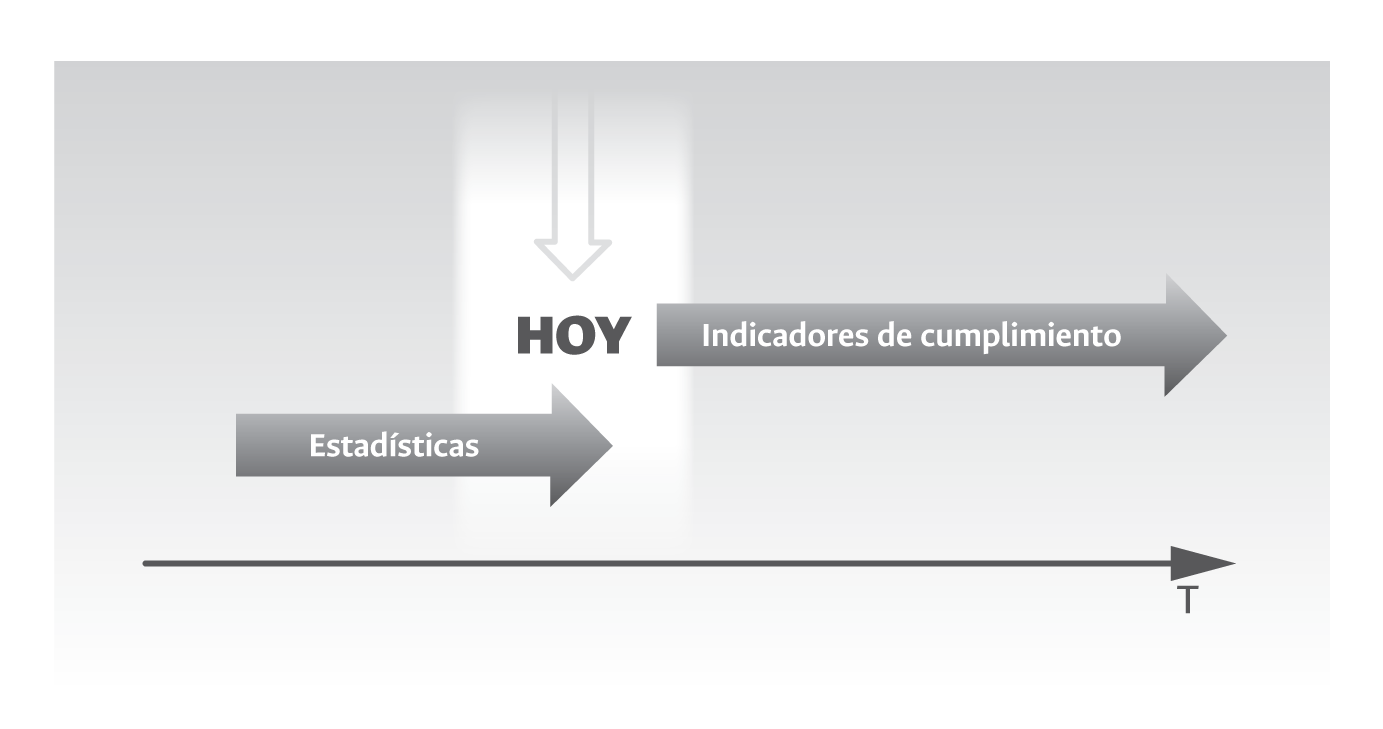
\includegraphics[width=0.75\linewidth]{imagenes/F_17} 

}

\caption{Contexto de las estadísticas y los indicadores a lo largo del tiempo. Fuente: elaboración propia.}\label{fig:fig17}
\end{figure}

\hypertarget{once-caracteruxedsticas-asociadas-a-las-estaduxedsticas}{%
\section[\textbf{Once características asociadas a las estadísticas}]{\texorpdfstring{\textbf{Once características asociadas a las estadísticas}\footnote{Esta caracterización de los rasgos que constituyen las estadísticas institucionales se soporta en la experiencia, los aportes y los lineamientos propios de la Universidad Nacional de Colombia. Más que una definición formal y de alcance global, se propone para ser analizada, adaptada, discutida y mejorada cuando así se considere en otras universidades y entidades públicas.}}{Once características asociadas a las estadísticas}}\label{once-caracteruxedsticas-asociadas-a-las-estaduxedsticas}}

Las estadísticas son cifras descriptivas de interés social e institucional que se caracterizan, en el ámbito de lo público y, dentro de este, en el contexto universitario, principalmente por:

\begin{enumerate}
\def\labelenumi{\arabic{enumi}.}
\tightlist
\item
  Ser construidas a partir de información poblacional o muestral obtenida de censos, registros administrativos o encuestas probabilísticas o no probabilísticas.
\item
  Estar conformadas por cifras agregadas de naturaleza descriptiva derivadas de conteos o de mediciones.
\item
  Caracterizar/desagregar temporal, temática y geográficamente rasgos de los individuos que conforman las poblaciones o muestras de interés.
\item
  Representar el presente y el pasado a través de la disposición de series de tiempo.
\item
  Tener la capacidad de reconocer y representar el comportamiento de grupos poblacionales minoritarios (incluyentes / inclusivas).
\item
  Ser susceptibles de ser representadas de manera tabular y gráfica (visualización).
\item
  Estar orientadas y delimitadas por normas y hacer uso de conceptos, estándares, clasificaciones y nomenclaturas internacionales, nacionales e institucionales que favorezcan su interpretación y comparación.
\item
  Estar disponibles a través de múltiples mecanismos de difusión y comunicación que permitan una adecuada interacción con los usuarios.
\item
  Hacer un uso intensivo de las nuevas tecnologías de la información y las comunicaciones.
\item
  Ser construidas a través de un proceso estadístico.
\item
  A partir de la comparación entre e intra poblaciones o muestras, aportar a la creación de nuevas estadísticas e indicadores institucionales y extrainstitucionales.
\end{enumerate}

\hypertarget{construidas-a-partir-de-informaciuxf3n-poblacional-o-muestral}{%
\chapter{\texorpdfstring{\textbf{\emph{Construidas a partir de información poblacional o muestral}}}{Construidas a partir de información poblacional o muestral}}\label{construidas-a-partir-de-informaciuxf3n-poblacional-o-muestral}}

La \emph{primera característica} de las estadísticas en el contexto de la universidad pública es que estas se extraen y soportan a partir de información disponible en poblaciones o muestras existentes a nivel institucional.

\textbf{\emph{Poblaciones}}

Es el tipo de información más frecuente de encontrar en el ámbito de la universidad pública para efectos de la construcción y consolidación de estadísticas institucionales. Según \citet{everitt2006cambridge}, el término población se usa para identificar la colección de unidades finitas e infinitas\footnote{En el contexto de la universidad pública es improbable encontrar ejemplos asociados a estadísticas derivadas de poblaciones infinitas, por lo que este documento, en adelante, cuando haga referencia al término población, asume que esta es finita, es decir, se conoce el número de individuos que conforman dichas poblaciones.} que corresponde muchas veces a personas pero que pueden ser también instituciones, eventos u otros. Las poblaciones de aspirantes a pregrado y posgrado, de estudiantes matriculados, de graduados, de revistas institucionales, de docentes de carrera, de funcionarios administrativos de carrera, etc., son ejemplos tangibles de poblaciones existentes en el contexto universitario las cuales, de hecho, soportan la construcción de estadísticas en la Universidad Nacional de Colombia dado el interés institucional existente por conocer el comportamiento global de ciertos aspectos comunes que comparten los individuos que las conforman\footnote{Los individuos que conforman una población, como su nombre probablemente lo sugiere, no se reducen a personas u otros seres vivos, sino que estos, en el ámbito de las poblaciones existentes al interior de las universidades públicas, incluyen también aquellos que se ubican fuera del contexto biológico. Revistas científicas, artículos, patentes, universidades con las que se tienen firmados convenios de doble titulación, empresas vinculadas a través de servicios de extensión, etc., son algunos ejemplos de poblaciones en donde claramente los individuos que las conforman no son seres vivos.}. Por ejemplo, es de interés institucional y social el conocimiento de la evolución histórica del total de aspirantes a cursar estudios de pregrado en la universidad, o ciertas características de estos como la edad, el sexo, la nacionalidad, el lugar de nacimiento, el estrato socioeconómico, entre otros.

Las características que comparten los miembros de una población de interés institucional son capturadas a través de lo que técnica y científicamente se conocen como \emph{variables}. Desde una perspectiva estadística, las variables\footnote{En un sentido coloquial una variable, como su nombre lo indica, hace referencia a algo que varía entre los individuos de una población o que puede estar sujeta a cambios. Por ejemplo, la edad es una variable asociada a poblaciones como los estudiantes, los aspirantes, los docentes, los graduados que, desde luego, varía entre los diferentes individuos que conforman dichas poblaciones.} asociadas a una población pueden ser clasificadas en: nominales, ordinales, de intervalo y de razón\footnote{Clasificación propuesta por \citet{stevens1946theory} en el artículo ``On the theory of scales of measurement'' de la revista \emph{Science}.} .

Las \emph{variables nominales}\footnote{También conocidas como variables categóricas.} son aquellas que permiten identificar cualidades de los individuos bajo observación. Por ejemplo, las variables sexo, estado civil y facultad en la que se encuentra matriculado un estudiante hacen parte del mundo de las variables nominales, las cuales se identifican/etiquetan con números o códigos cuyo único propósito es poder asociar una cualidad observada en los individuos, no es una característica numérica de estos. Las \emph{variables ordinales}, a diferencia de las nominales, tienen un orden establecido; el estrato socioeconómico de un estudiante y el máximo nivel de formación alcanzado por un docente, por ejemplo, hacen parte del mundo de las variables ordinales. Tener como máximo nivel de formación pregrado es menor que tener maestría y este, desde luego, es menor que tener estudios de doctorado. Las variables nominales y ordinales hacen uso de los números con propósitos de identificación de cualidades, no obstante, en estas últimas existe una relación de orden entre dichas cualidades.

Las \emph{variables de razón y de intervalo} hacen uso de los números para representar características asociadas a los individuos que conforman una población o muestra de interés. La única diferencia existente entre estos dos tipos de variables es el cero absoluto. En las variables de razón el cero significa ausencia de un atributo de interés, mientras que en las de intervalo el cero no significa la ausencia de dicho atributo. El tiempo de vinculación de un docente de carrera en la universidad, y el puntaje obtenido por los estudiantes en una prueba de admisión son dos ejemplos de variables de razón, dado que el valor cero significa que hasta ahora se vincula un docente a la universidad o que se obtuvo un valor de cero en una prueba de admisión --la peor puntuación--. La temperatura en un día dado, en contraste, es el ejemplo clásico empleado para representar variables de intervalo puesto que el valor cero no significa ausencia de atributo; es decir que no exista temperatura.

El mundo de las variables nominales y ordinales, dado el uso que hacen de los números, conforma lo que popularmente se conoce como variables de tipo cualitativo\footnote{El uso del término cualitativo en el contexto estadístico no debe confundirse con el uso de este término en el estudio de fenómenos sociales que hacen uso de técnicas y métodos de tipo cualitativo y, en especial, aquellas empleadas por disciplinas de las ciencias humanas y sociales.}. Por su parte, el escenario de las variables de razón y de intervalo, dada su naturaleza numérica asociada, conforman el mundo de las variables cuantitativas. Los métodos y las técnicas estadísticas y analíticas deben su origen y se justifican gracias a su poder para estudiar los diversos fenómenos de estos dos conjuntos de variables. Unos son los métodos estadísticos y de analítica de datos disponibles para el estudio de fenómenos, que incluyen variables cualitativas, y otros aquellos disponibles para el estudio de las variables cuantitativas. La construcción de estadísticas institucionales se soporta principalmente en la disposición y construcción de variables de tipo cualitativo.

\begin{itemize}
\tightlist
\item
  \emph{Tipos de poblaciones}
\end{itemize}

Las estadísticas asociadas a información de tipo poblacional pueden ser de naturaleza diversa de acuerdo con la forma como son obtenidas o consolidadas. En principio, y salvo contadas excepciones, estas pueden ser de tipo transversal, anidado o longitudinal.

Las \emph{poblaciones de tipo transversal}, como se ilustra en la figura \ref{fig:fig18}, son aquellas obtenidas en un punto determinado del tiempo sin importar el momento en que los individuos que las conforman empezaron a ser parte de las mismas. Para el caso de las universidades, los momentos típicos de corte empleados para la obtención y consolidación de poblaciones con propósitos de construcción de estadísticas son los semestres y los años\footnote{En otras áreas de interés social se requieren periodos más cortos para la consolidación de poblaciones con miras a la disposición de estadísticas. Por ejemplo, en el contexto económico colombiano actual algunas cifras de interés nacional, como el Índice de Precios al Consumidor (IPC) y las tasas de desempleo se calculan y disponen de manera mensual por parte del DANE y el Banco de la República, respectivamente.}. Por ejemplo, en la Universidad Nacional de Colombia, poblaciones como las de aspirantes a pregrado y posgrado, de admitidos a pregrado y posgrado, de estudiantes matriculados, de graduados, de estudiantes en movilidad internacional, de funcionarios administrativos, de docentes, etc., se obtienen semestralmente con el fin de consolidar las estadísticas institucionales asociadas a estas. Poblaciones relacionadas con la investigación, dado su comportamiento, se obtienen anualmente.

\begin{figure}

{\centering 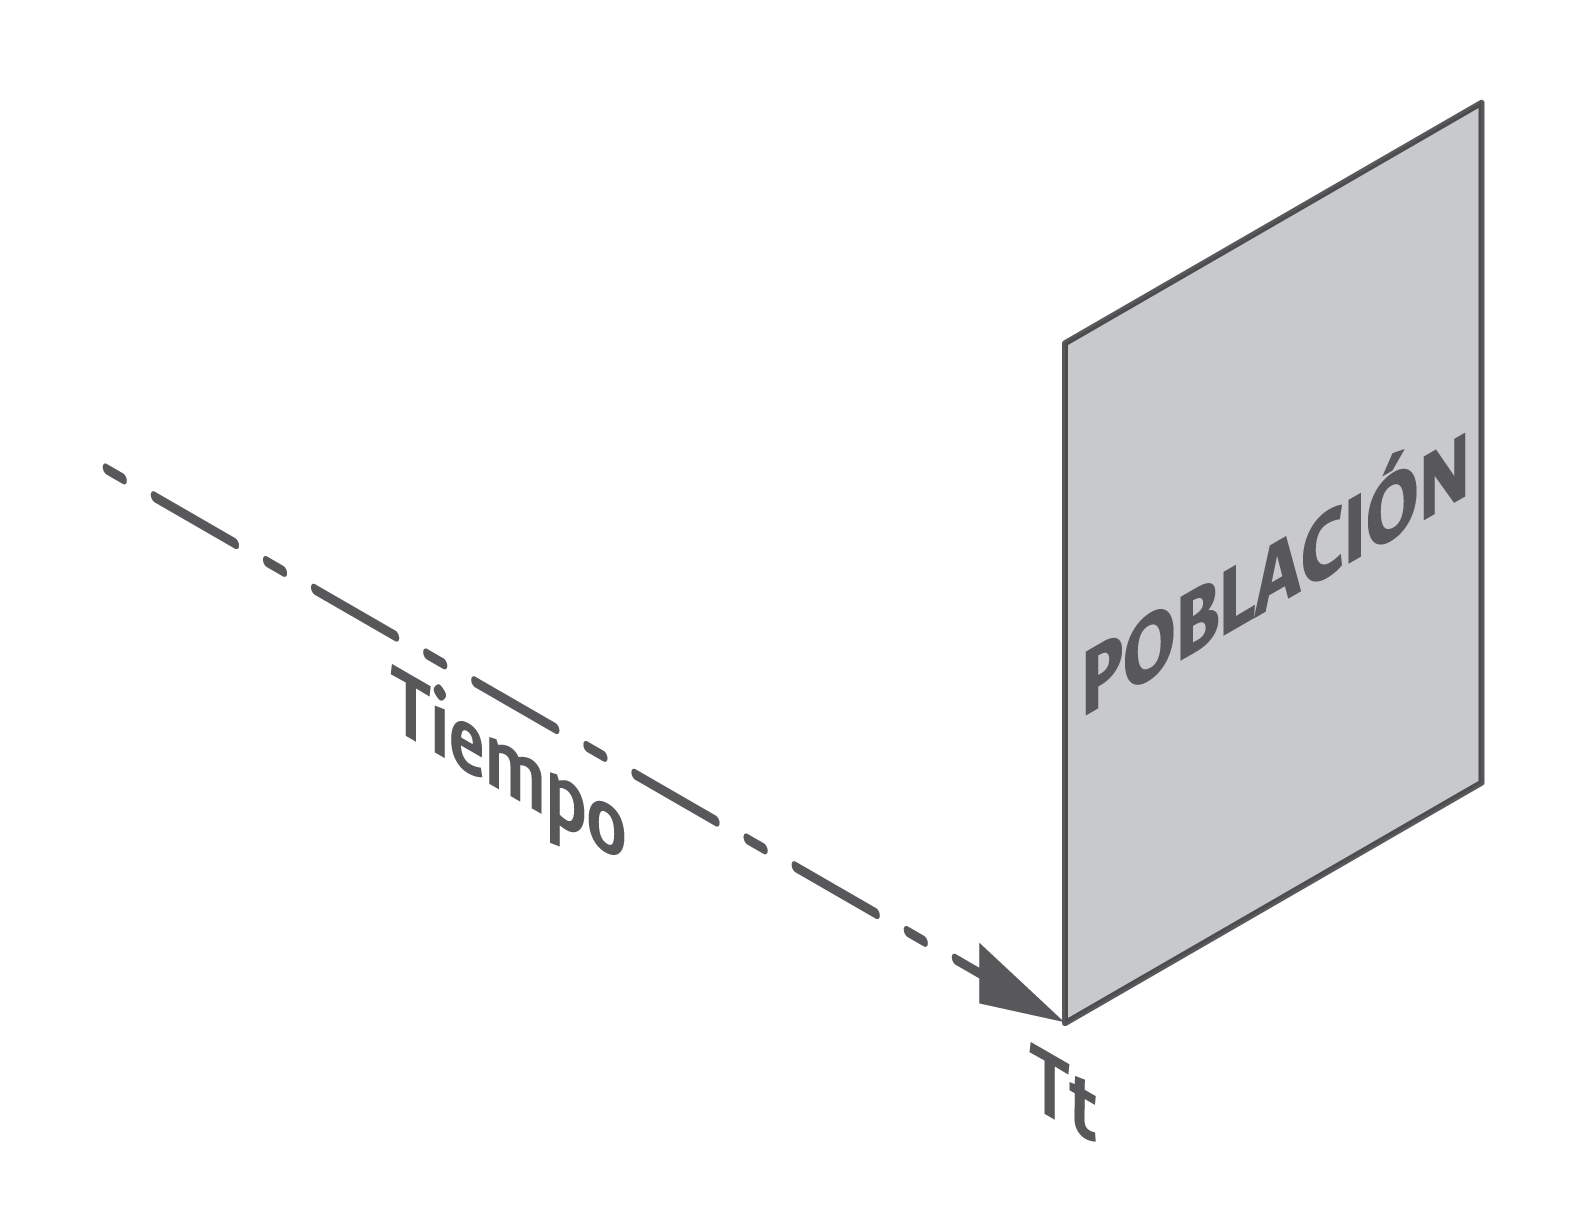
\includegraphics[width=0.75\linewidth]{imagenes/F_18} 

}

\caption{Representación esquemática de una población de tipo transversal. Fuente: elaboración propia.}\label{fig:fig18}
\end{figure}

Las \emph{poblaciones de tipo anidado} también se obtienen en un punto determinado del tiempo sin importar el momento en que los individuos que las conforman empezaron a ser parte de estas. No obstante, estas poblaciones a su vez están contenidas dentro de una población mayor (figura \ref{fig:fig19}) de la cual y contra la cual se extrae información de interés para las estadísticas institucionales. Las poblaciones de estudiantes admitidos o de matriculados por primera vez son ejemplos típicos de poblaciones anidadas, pues estas se encuentran contenidas dentro de una población mayor que es la de aspirantes (para el caso de los admitidos) y la de matriculados (para el caso de los matriculados por primera vez). Las poblaciones anidadas, además de servir de base para la consolidación de estadísticas, favorecen la construcción de indicadores simples como el de cobertura de admitidos a pregrado y posgrado en las universidades públicas (proporción entre admitidos y aspirantes).

\begin{figure}

{\centering 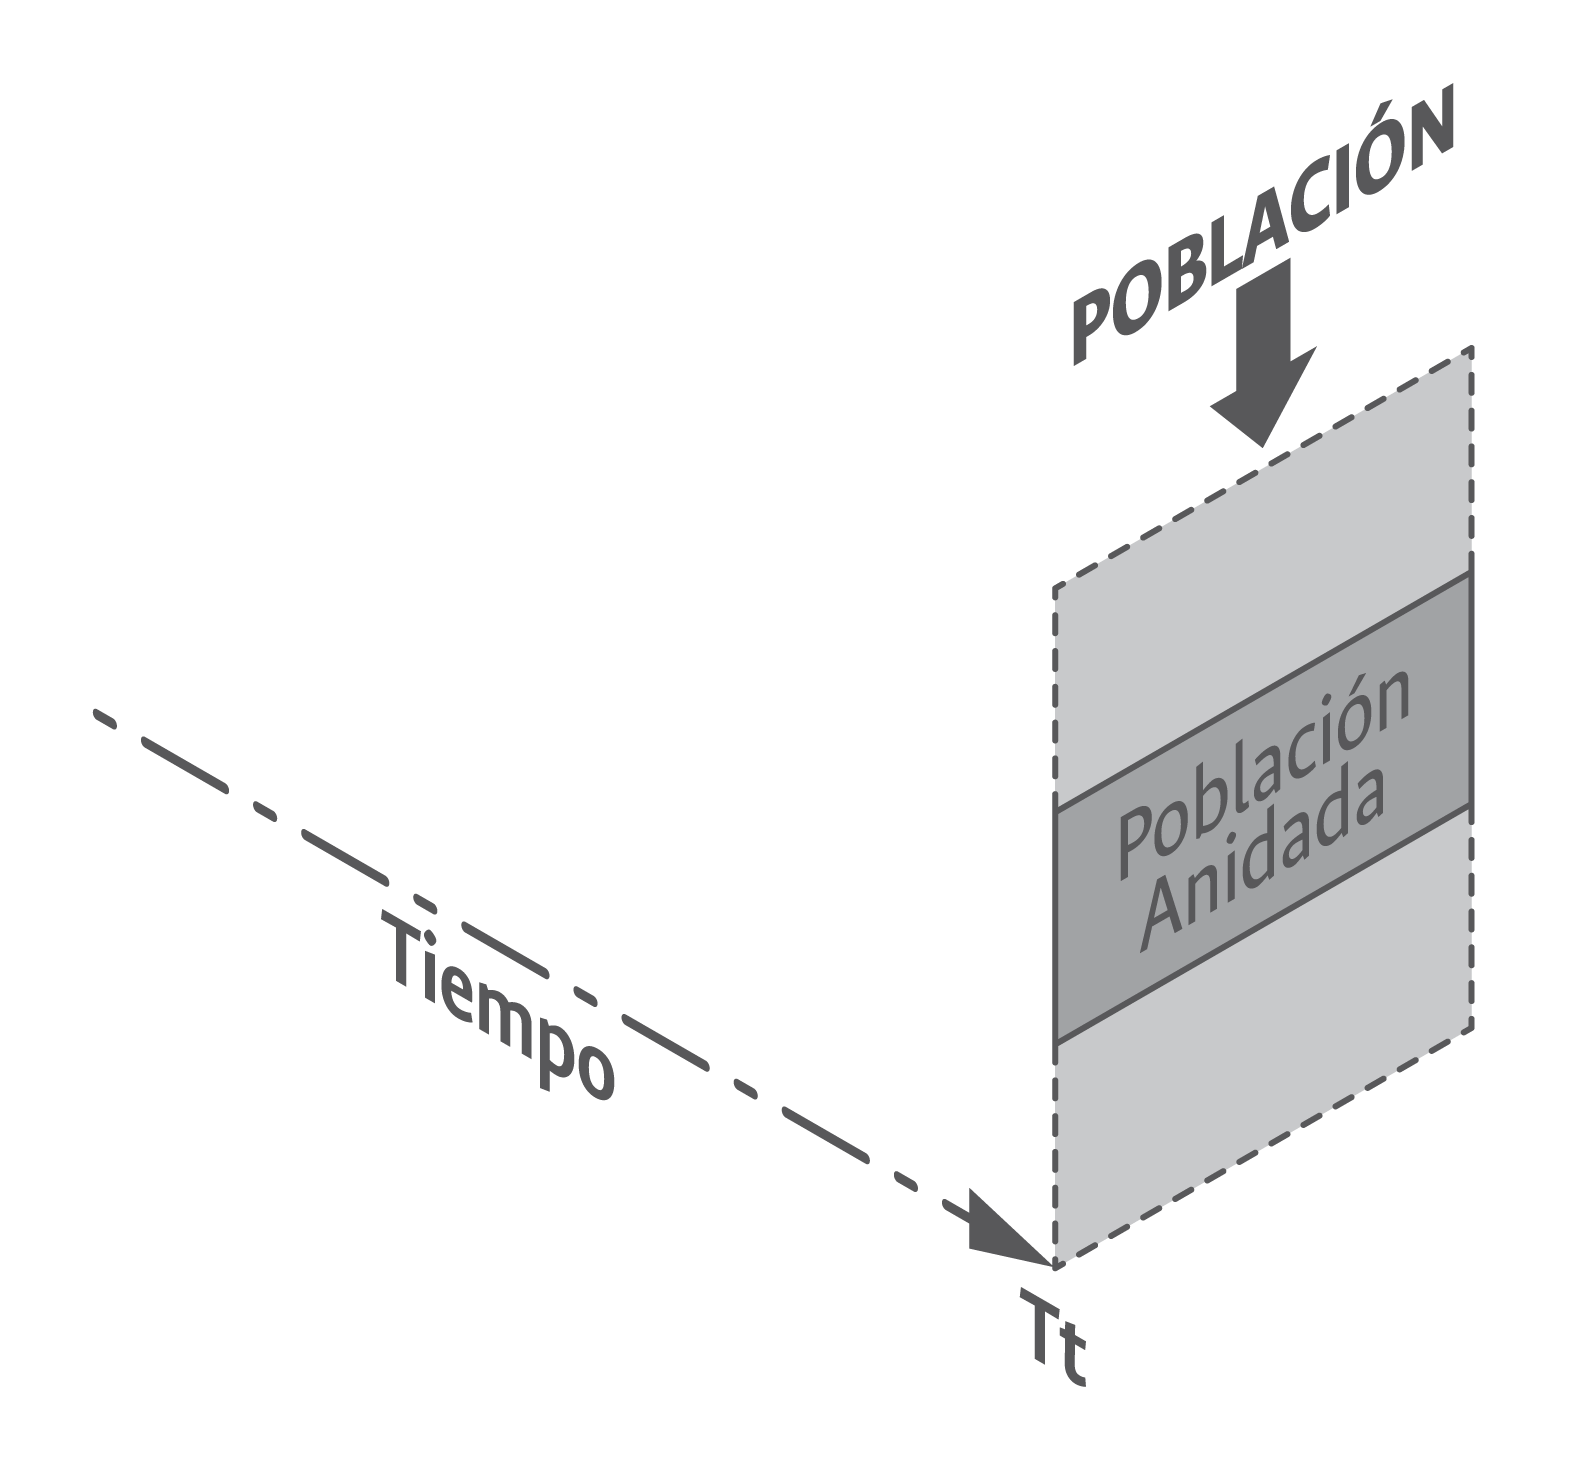
\includegraphics[width=0.75\linewidth]{imagenes/F_19} 

}

\caption{Representación esquemática de una población de tipo anidado. Fuente: elaboración propia.}\label{fig:fig19}
\end{figure}

Las \emph{poblaciones de tipo longitudinal} son aquellas obtenidas en un momento del tiempo en las cuales, a diferencia de las poblaciones transversales y anidadas, sí importa el tiempo en que los diferentes individuos que las conforman empezaron a ser parte de estas. Aunque teóricamente el tiempo de ingreso a la población de estudio puede ser medido de manera precisa, para el caso de la información de las universidades es frecuente que este sea igual para un número elevado de individuos y conforma lo que metodológicamente se conoce como cohortes\footnote{Aunque existe una amplia variedad de definiciones sobre el significado de cohorte, para propósitos de este documento las entendemos como un grupo de individuos que son objeto de estudio a lo largo del tiempo, y que se caracterizan porque se conoce el momento en el que estos empezaron a conformarlas, así como la evolución de sus respectivas características.}. Por ejemplo, la población conformada por la unión de las cohortes de estudiantes admitidos a pregrado durante varios periodos de tiempo, además de permitir la consolidación de estadísticas institucionales, es la base para la construcción y medición de indicadores complejos como las tasas de deserción universitaria en las cuales se ha demostrado que el tiempo juega un rol fundamental. En la figura \ref{fig:fig20} se puede observar que la población ilustrada en un momento o periodo del tiempo, está conformada por los individuos que integran un número de diferentes cohortes de interés institucional.

\begin{figure}

{\centering 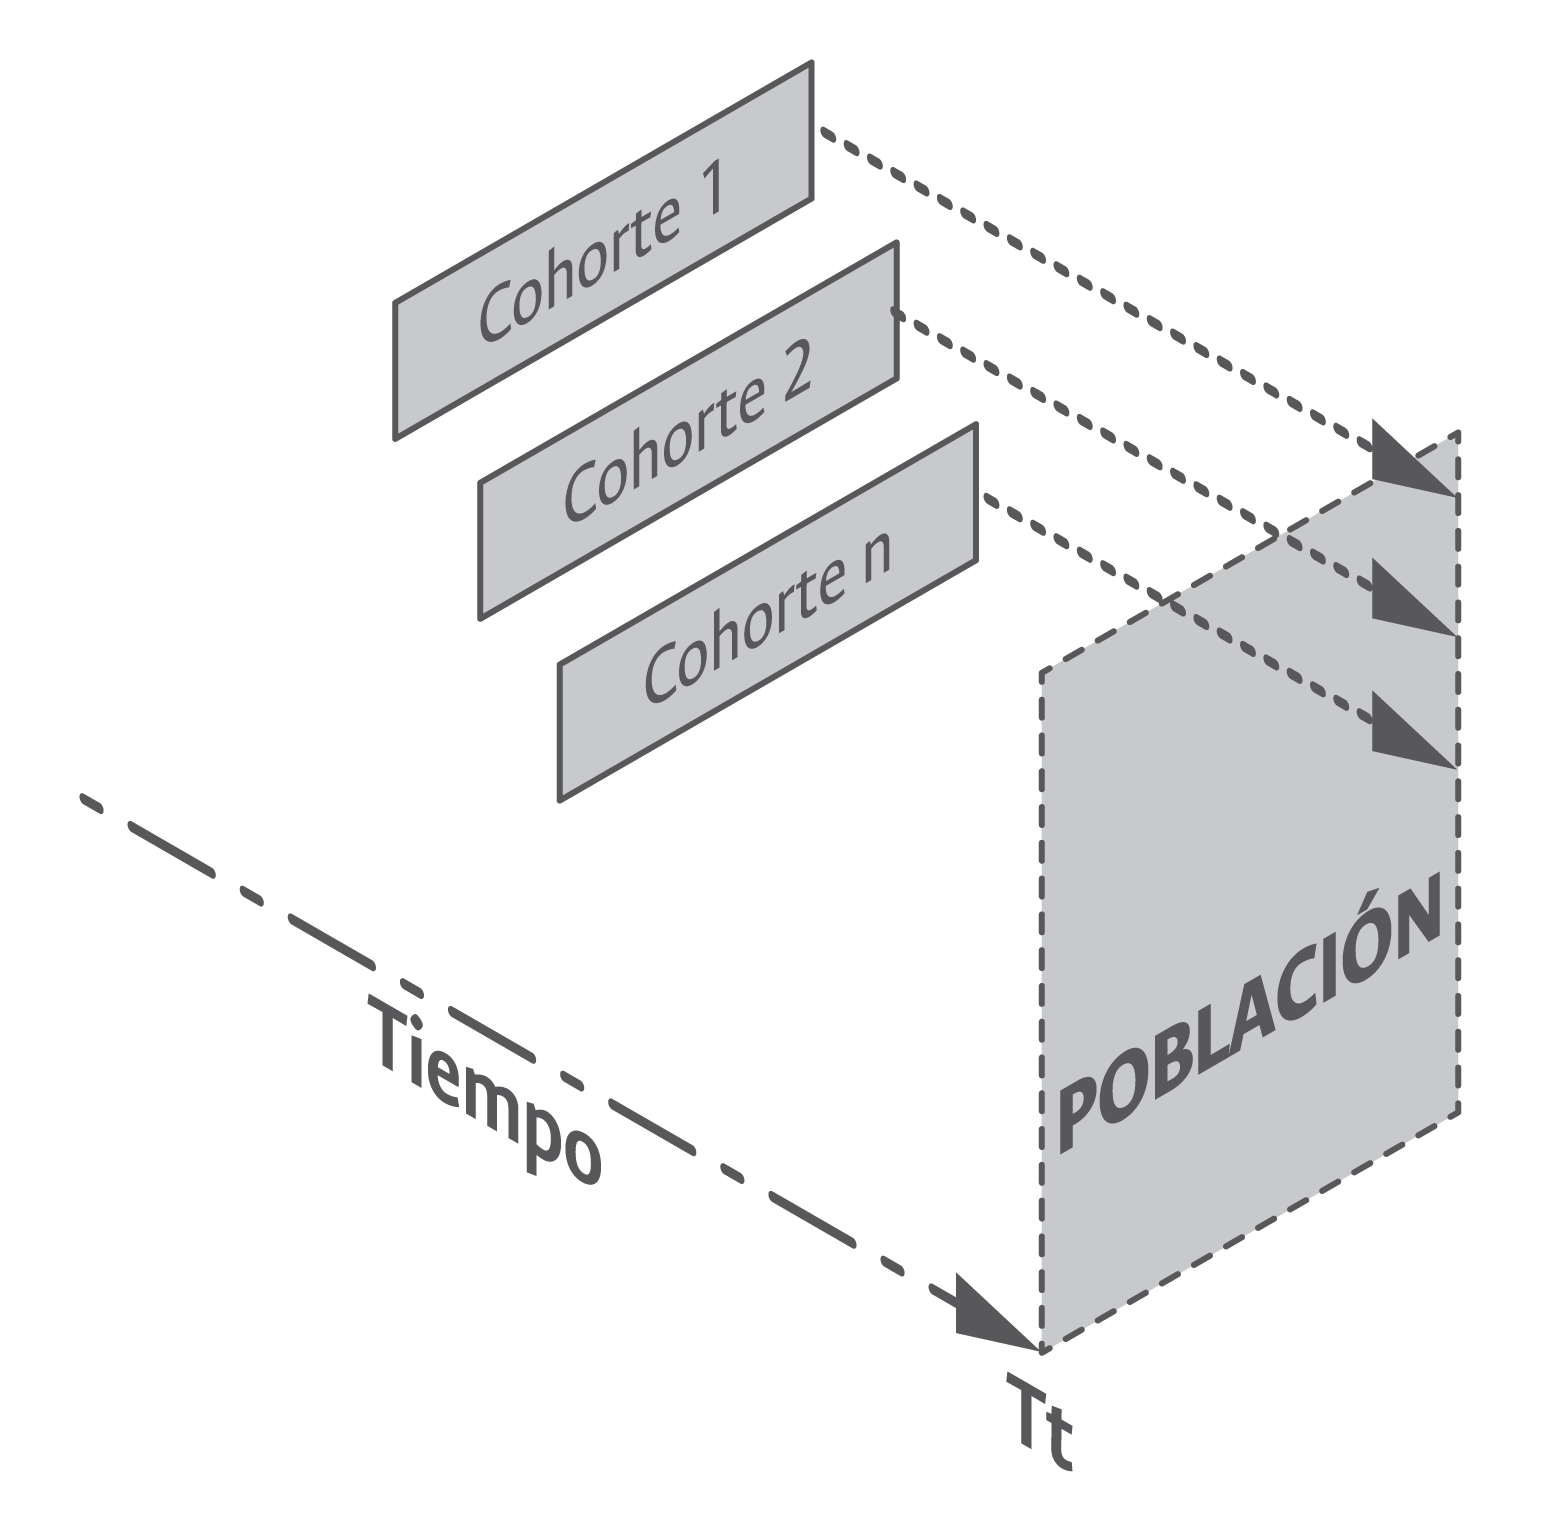
\includegraphics[width=0.75\linewidth]{imagenes/F_20} 

}

\caption{Representación esquemática de una población de tipo longitudinal. Fuente: elaboración propia.}\label{fig:fig20}
\end{figure}

\begin{itemize}
\tightlist
\item
  \emph{Disposición de poblaciones}
\end{itemize}

En el escenario de la universidad actual existen dos mecanismos de conformación de poblaciones: los registros administrativos y los censos.

El Estado y sus instituciones, desde la misma conformación de las naciones modernas, han sido grandes acopiadores y usuarios de información estadística de alcance poblacional. La forma como esta es capturada y almacenada se materializa en la actualidad, según el DANE, a través del uso de los \emph{registros administrativos}, entendidos como: ``Toda información que las instituciones públicas o privadas recolectan, almacenan o administran de personas naturales o jurídicas, en el ejercicio de sus funciones o competencias''\footnote{Artículo 1.3.1.1 del Decreto 1743 de 2016 del DANE.}. La información poblacional de estudiantes matriculados, de docentes y funcionarios, de grupos de investigación, de profesores visitantes, entre otros, que es obtenida con propósitos administrativos, que se gestiona al interior de las universidades a través de sistemas de información y que se encuentra disponible en bases de datos institucionales, es información poblacional obtenida a través del uso de registros administrativos.

Un segundo mecanismo de acceso a información poblacional son los \emph{censos}\footnote{Los censos son el método estadístico más antiguo empleado por la humanidad para la obtención de información cuantitativa, como lo demuestra su uso desde tiempos bíblicos, por ejemplo, Lucas 2:1 cita: ``Y aconteció en aquellos días que salió un edicto de César Augusto, para que se hiciera un censo de todo el mundo habitado''. Otros ejemplos de apartados bíblicos en el que se hace alusión de manera directa o indirecta a información censal son: Números 1:2, Números 3:40, Jueces 21:9, Samuel 11:18, Samuel 13:15, Isaías 33:18, Samuel 24:4, etc., y hacia el año 2238 antes de la era cristiana en la China al mando del emperador Yao. Desde los inicios de la nueva era cristiana, pasando por la Edad Media, el Renacimiento y hasta la consolidación y conformación de las naciones actuales, los censos, en especial aquellos asociados a las poblaciones humanas, siguen siendo uno de los instrumentos empleados de manera regular para la obtención y consolidación de estadísticas nacionales y la construcción de información clave para la disposición y medición de indicadores sectoriales e institucionales.} . A través de esta metodología se observa a cada miembro de una población con el fin de extraer de ellos información de interés de un conjunto de variables para su posterior análisis e interpretación.

Los censos, de amplio uso en el ámbito nacional, son poco frecuentes en el contexto de las instituciones públicas para la conformación de poblaciones con miras a la consolidación de estadísticas institucionales. El poco uso de este mecanismo de obtención de información poblacional en el ámbito de las universidades se debe en especial a la buena disposición de datos a través del uso de registros administrativos la cual, además de implicar bajos costos y despliegues administrativos, se encuentra disponible de manera periódica, lo que no ocurre con los censos.

\textbf{\emph{Muestras}}

La construcción y consolidación de estadísticas de alcance poblacional es el fin buscado en el ámbito de lo público. Esta información se obtiene a través del uso de registros administrativos o de censos cuando las circunstancias lo permiten (objetivos globales, poblaciones relativamente pequeñas y fácilmente identificables, recursos suficientes, etc.) (\citet{sarndal2003model}; \citet{soto1996fundamentos}). No obstante, en ocasiones se requiere cierta información y, por diversas razones, no es factible acceder a todos los individuos que conforman las poblaciones. Para estos casos, el mecanismo de obtención de información tradicionalmente empleado son las muestras\footnote{Las muestras, al igual que las poblaciones, pueden ser clasificadas según su naturaleza en transversales, anidadas y longitudinales.}.

Una muestra está conformada por un subconjunto de individuos de una población, los cuales pueden o no ser seleccionados a través de un mecanismo probabilístico. En las muestras, al igual que en las poblaciones, los individuos comparten características comunes sobre las que se está interesado en obtener estadísticas poblacionales de interés nacional, sectorial o institucional haciendo uso para ello de estimaciones inferidas a partir de los comportamientos observados en los individuos que las conforman. Una \emph{muestra probabilística}\footnote{El muestreo probabilístico o estadístico conforma un área de estudio de la disciplina estadística contemporánea, el cual cuenta con importantes desarrollos teóricos y metodológicos, así como una alta popularidad y uso en el contexto de la práctica estadística moderna, gracias a la precisión alcanzada.}, según \citet{levy2013sampling}, es aquella en donde los individuos que la conforman fueron seleccionados a través de un procedimiento en el cual cada uno de aquellos que conformaban la población finita de origen tenía una probabilidad conocida (no necesariamente igual) de ser seleccionados. En caso contrario, \emph{la muestra es no probabilística}.

Un ejemplo del uso de muestras para la consolidación de estadísticas institucionales en el contexto de la educación superior son los llamados indicadores de opinión requeridos por el CNA en el marco de las autoevaluaciones con fines de acreditaciones de alta calidad. Los indicadores de opinión hacen referencia principalmente a la apreciación de estudiantes, egresados y docentes sobre aspectos académicos y administrativos del quehacer de las instituciones y sus programas académicos para los cuales, en la mayoría de los casos, no se cuenta con información poblacional accesible a través de registros administrativos y, por consiguiente, es común que se acceda a la misma a través del uso de muestras que regularmente son conformadas y construidas a través del uso de estrategias no probabilísticas, a pesar de la disposición de marcos poblacionales institucionales.

\hypertarget{conformar-cifras-agregadas}{%
\chapter{\texorpdfstring{\textbf{\emph{Conformar cifras agregadas}}}{Conformar cifras agregadas}}\label{conformar-cifras-agregadas}}

La \emph{segunda característica} de las estadísticas está relacionada con la capacidad que estas tienen para representar la información de manera resumida o agregada. Las estadísticas no existen sin la disponibilidad de cifras descriptivas agregadas, producto de la actividad de contar o de medir, estas son su esencia. Las estadísticas se interesan por el descubrimiento de regularidades sociales, no es de su interés el estudio del comportamiento de rasgos individuales, aunque se valen de ellos para sus propósitos\footnote{El ejercicio estadístico moderno, en el contexto de la construcción y consolidación de estadísticas nacionales e institucionales, se fundamenta en la otrora disciplina estadística de mediados del siglo pasado cuyo interés se centraba principalmente en el estudio de estos tipos de medidas y en especial aquellas requeridas y asociadas al contexto de los Estados. De hecho, en 1940 se definía a la disciplina estadística como ``el cómputo o enumeración metódica de los hechos, de los individuos o de las cosas que pueden contarse o medirse y la coordinación de las cifras obtenidas'', en donde por coordinación se entendía ``la aproximación, la comparación y el arreglo de las cifras, bajo la forma de cuadros y gráficos, para facilitar la utilización de ellas con fines prácticos y científicos'' (\citet{rodriguez}, p.~16). Hoy, la disciplina estadística se ha acercado de manera importante a la línea matemática y científica en detrimento de la de mediados del siglo pasado, la cual podríamos catalogar como una estadística de naturaleza administrativa.}.

Las medidas agregadas asociadas a las estadísticas son aproximaciones de tipo descriptivo que pueden ser de dos tipos: conteos o mediciones.

\begin{itemize}
\tightlist
\item
  \emph{Conteos: estadísticas derivadas de variables cualitativas}
\end{itemize}

El primer tipo de cifras derivadas del proceso de construcción de estadísticas lo conforman aquellas cuyo resultado es el producto de contar los individuos que conforman una población o muestra, o que al interior de estas comparten ciertos rasgos o atributos de interés. Por ejemplo, el total de estudiantes matriculados en un momento dado del tiempo y, de estos, cuántos son hombres, cuántas son mujeres, cuántos pertenecen a un estrato socioeconómico bajo, cuántos están ubicados en una determinada sede o facultad, etc., es el resultante de una actividad centrada en contar individuos y rasgos de estos al interior de una población la cual, en el caso de nuestro ejemplo, está conformada por los estudiantes matriculados en una universidad.

Las medidas estadísticas agregadas, producto de la actividad de contar, se construyen a partir de la disposición de variables nominales u ordinales. La construcción y disposición de estas variables ofrecen una gran posibilidad para contar y para construir series, a través de las cuales es posible observar los cambios y las tendencias que sufren las cifras a lo largo del tiempo. Esto último nos lleva a concluir que la construcción de estadísticas es más una actividad de cuantificación que de medición en sentido estricto; es decir, contar pero, sobre todo, contar bien, y para ello es suficiente con tener buenas nociones sobre los tipos de variables y las operaciones básicas de la aritmética\footnote{Aunque el conteo es el ideal buscado, no siempre, por cuestiones técnicas o por exigencias institucionales, es posible alcanzarlo, en cuyo caso debemos acudir a las mediciones. Medir, desde luego, es tan importante en el contexto de la consolidación y construcción de estadísticas como contar.}.

\begin{itemize}
\tightlist
\item
  \emph{Mediciones: estadísticas derivadas de variables cuantitativas}
\end{itemize}

El segundo tipo de cifras asociadas a la construcción de estadísticas lo conforman aquellas que miden ciertos parámetros de interés poblacional asociados al comportamiento de los individuos en una o más variables de interés. Mientras que el primer tipo de cifras asociadas a las estadísticas se centra en contar, este tipo de cifras se centra en medir, por ejemplo, las medidas de tendencia central como el promedio, la mediana o la moda; de posición no central como los cuartiles, deciles, quintiles o percentiles; de dispersión como la varianza, la desviación estándar o el rango; de apuntamiento como la kurtosis, y de simetría o asimetría.

La medición en el contexto de las estadísticas exige el uso y la disposición de variables cuantitativas al interior de las poblaciones que las soportan. A partir de este tipo de variables es posible construir cifras estadísticas agregadas que miden comportamientos globales de interés. Por ejemplo, en el contexto universitario, el promedio de edad de los estudiantes, su varianza, los cuartiles en las que estas se ubican, así como la asimetría observada hacen parte de las probables cifras estadísticas de naturaleza descriptiva que pueden medir estos parámetros de interés institucional.

\begin{itemize}
\tightlist
\item
  \emph{Transformación entre tipos de variables}
\end{itemize}

Las tipologías de las variables asociadas a una población o muestra, en el marco de la construcción de estadísticas, pueden ser transformadas en nuevas tipologías a través de un ejercicio de mutación de valores originales en nuevos valores. No obstante, no toda tipología de una variable puede ser transformada en una nueva tipología pues estas presentan ciertas reglas. La principal regla es la \emph{imposibilidad de transformar variables cualitativas en cuantitativas}. La segunda regla es la \emph{posibilidad de transformar variables cuantitativas en cualitativas, pero a lo sumo dentro de estas en variables ordinales}\footnote{Existen más reglas de transformación de los tipos de variables, por ejemplo, la posibilidad de transformar variables nominales en variables dicotómicas o \emph{dummies}. El presente trabajo, por utilidad directa con el proceso de construcción de estadísticas, presenta únicamente dos reglas de transformación.}. Por ejemplo, desde una perspectiva estadística, la edad de un estudiante es una variable cuantitativa de razón, la cual puede ser transformada en una variable cualitativa ordinal a partir de la creación de clases o rangos de edad a la cual pertenecen las respectivas edades. En este sentido, un estudiante de pregrado con una edad de 17,5 años puede pertenecer a la clase de estudiantes con 18 años o menos, mientras que uno con 23 años puede pertenecer al grupo de estudiantes con 22 o más años y así sucesivamente, sin olvidar que cada una de las edades debe pertenecer a una única clase.

La posibilidad de transformar variables cuantitativas en variables cualitativas favorece el proceso de construcción de estadísticas y debe ser usada si las circunstancias técnicas y funcionales lo permiten.

\hypertarget{caracterizar-y-desagregar-rasgos-de-interuxe9s-de-los-individuos-que-conforman-las-poblaciones-o-muestras}{%
\subsection{\texorpdfstring{\textbf{\emph{Caracterizar y desagregar rasgos de interés de los individuos que conforman las poblaciones o muestras}}}{Caracterizar y desagregar rasgos de interés de los individuos que conforman las poblaciones o muestras}}\label{caracterizar-y-desagregar-rasgos-de-interuxe9s-de-los-individuos-que-conforman-las-poblaciones-o-muestras}}

La \emph{tercera característica} de las estadísticas es la \emph{capacidad de disponer y presentar información de manera desagregada}. En el apartado anterior se expuso que esta información se encuentra contenida en las variables disponibles en una población o muestra de origen. Las variables que conforman una población o muestra, para propósitos de construcción y disposición de estadísticas, pueden ser clasificadas a su vez según la posibilidad que estas tienen para representar la información de interés institucional desde diferentes perspectivas conocidas como desagregaciones. Las desagregaciones a través de las cuales se representa la información institucional, en el contexto de la universidad pública, son de tres tipos: temporales, geográficas/institucionales y temáticas.

\begin{itemize}
\tightlist
\item
  \emph{Desagregaciones temporales}
\end{itemize}

Una característica central de las estadísticas es la capacidad que tienen para representar la información desde una perspectiva temporal. En una universidad, por ejemplo, es tan importante conocer el número de matriculados en un momento dado del tiempo como su evolución histórica. La capacidad de las estadísticas para representar la información desde una perspectiva histórica implica la consolidación, el almacenamiento y la disposición de las poblaciones y muestras generadas a lo largo del tiempo. Los años, los semestres y, en una menor medida, los trimestres o meses son las variables comúnmente empleadas en el ámbito de la universidad colombiana para la provisión de estadísticas desde una perspectiva temporal\footnote{Aunque en la teoría existe, y técnicamente hoy día es factible contar con información en tiempo real, para el caso de las estadísticas de una universidad pública es tolerable que estas estén medidas en periodos de tiempo que implican algunos rezagos en el acceso y la disposición de información institucional como son los semestres o los años.}, y que conforman el subconjunto de desagregaciones temporales contenidas dentro de las poblaciones o muestras que las conforman.

\begin{itemize}
\tightlist
\item
  \emph{Desagregaciones geográficas e institucionales}
\end{itemize}

Los individuos que conforman una muestra o población asociada a la construcción de estadísticas generalmente se encuentran distribuidos espacialmente dentro de un territorio o ubicados jerárquicamente dentro de una estructura organizacional. La capacidad de las estadísticas para representar la información desde una perspectiva geográfica o institucional es una de las características esenciales que favorecen el hacer y la toma de decisiones en el contexto de lo público. Para una universidad como la Nacional es tan importante saber, por ejemplo, de qué municipios y departamentos del país proceden los estudiantes matriculados en un momento dado del tiempo como de qué países son los títulos obtenidos por sus docentes en sus máximos niveles de formación. Así mismo, a nivel institucional, es tan importante saber cuántos estudiantes están matriculados en una de sus sedes como el conocimiento sobre la distribución de estos por las respectivas facultades, institutos, escuelas y programas académicos de dichas sedes.

Las \emph{desagregaciones geográficas nacionales e internacionales} hacen un uso intensivo de información georreferenciada estandarizada a través de la cual es posible representar y comparar la información estadística institucional desde una perspectiva territorial. Las codificaciones estandarizadas de países, las distancias angulares de longitud y de latitud asociadas a un punto en un territorio particular, así como la disponibilidad de polígonos que representan áreas de interés nacional como los municipios o los departamentos hacen parte de los estándares requeridos para la disposición de estadísticas desde una perspectiva geográfica. En el módulo de cifras del sitio web de estadísticas de la Universidad Nacional de Colombia\footnote{Ver UN - Cifras, en \url{http://estadisticas.unal.edu.co/index.php?id=13}} podrán ser exploradas, para el caso de poblaciones como los aspirantes y admitidos a pregrado y posgrado, los matriculados, los graduados y los docentes de carrera, representaciones geográficas a través de la disposición de mapas web interactivos con la distribución de estas poblaciones según el territorio en el que han nacido, proceden, residen o han alcanzado máximos niveles de formación, por ejemplo\footnote{Esta información implica decisiones institucionales. Si, por ejemplo, se llegara a detectar que la población de aspirantes y admitidos a pregrado en la Universidad Nacional de Colombia se concentra solo en unos pocos municipios o departamentos del país, se podrían tomar medidas que permitan reiterar su carácter nacional.}.

Además de la necesidad de disponer de información estadística desde un ámbito nacional e internacional, es de interés institucional que la información cuantitativa disponible tenga la capacidad de ser presentada desde una perspectiva interna --geografía institucional--. La forma como se organizan las universidades\footnote{La Constitución Política de Colombia de 1991 reconoce la autonomía universitaria a todas las universidades del país, esto, a diferencia de otras entidades del Estado, les permite definir de manera libre la forma como se organizan y prestan el servicio público de educación superior.} difiere de manera importante, hecho que exige de las estadísticas el uso de normas internas que favorezcan la desagregación y presentación de la información cuantitativa desde una perspectiva organizacional.

La organización y presentación de las estadísticas en una universidad debe tener la capacidad de reconocer, cuando así se requiera, la forma como estas se organizan. Por ejemplo, la Universidad Nacional de Colombia, según su Estatuto General\footnote{Expedido mediante el Acuerdo 11 de 2005 del CSU, en \url{http://www.legal.unal.edu.co/rlunal/home/doc.jsp?d_i=35137}}, se organiza académica y administrativamente en la actualidad en tres niveles: nivel nacional, nivel de sede y nivel de facultad, los cuales a su vez se subdividen en otros niveles. La Universidad tiene en la actualidad nueve sedes físicas ubicadas a lo largo del territorio nacional\footnote{Bogotá, Medellín, Manizales, Palmira, Caribe, Orinoquia, Amazonia, Tumaco y La Paz.}, hecho que exige el reconocimiento de sus particularidades y el fomento del uso y la disposición de la información cuantitativa que obedezca a la cultura de cada una de sus sedes. En esta universidad es tan importante contar con información cuantitativa a través de estadísticas a nivel nacional --el todo-- como disponer de esta misma o nueva información en cada una de sus sedes. Por lo anterior, la apuesta actual de consolidación de un sistema estadístico a nivel institucional tiene entre sus retos ser capaz de representar la información de manera organizada tanto a nivel nacional como a través de cada una de sus sedes, y al interior de estas entre las facultades, escuelas y departamentos. A la fecha, además de la información oficial, estratégica y nacional contenida en el sitio web de estadísticas de esta universidad\footnote{Ver UN en un vistazo, en \url{http://estadisticas.unal.edu.co/}}, existen importantes ejercicios de consolidación de esta misma idea y de fomento de la cultura estadística en las sedes de esta institución, como lo evidencian los trabajos adelantados en este sentido en Bogotá\footnote{Ver UN - La sede en cifras, en \url{http://planeacion.bogota.unal.edu.co/cifras.html}}, Medellín\footnote{\url{http://planeacion.medellin.unal.edu.co/} opción ESTADISTICA} y Orinoquia\footnote{Ver Boletín Estadístico de la Sede Orinoquia, en \url{https://estadisticaun.github.io/BoletinOrinoquia/index.html}}, principalmente.

\begin{itemize}
\tightlist
\item
  \emph{Desagregaciones temáticas}
\end{itemize}

Las desagregaciones temáticas son características de los individuos que hacen parte de poblaciones o muestras las cuales trascienden el tiempo y la geografía y, al igual que estas, hacen parte constitutiva de las estadísticas. Por ejemplo, el sexo, el género, la edad, las condiciones socioeconómicas, la presencia de discapacidades, entre otras, hacen parte de los tipos de desagregaciones probables de ser tenidas en cuenta en las universidades para caracterizar las poblaciones humanas que hacen parte de sus comunidades.

Para la Universidad Nacional de Colombia, por ejemplo, son de interés desagregaciones temáticas de la estadística de aspirantes a pregrado: la presencia o ausencia de discapacidades, tipos de inscripción, nacionalidad, edad, estrato, sexo, puntajes en la prueba de admisión, tipo de inscripción, modalidades de inscripción, admitidos, pertenencia a programas de admisión especial, entre otras. Para el caso de las estadísticas de docentes, en esta institución las desagregaciones temáticas de interés son la edad, el sexo, la nacionalidad, el máximo nivel de formación, la dedicación, los años de servicio y la categoría docente. Cada población o muestra asociada a las estadísticas institucionales posee desagregaciones temáticas y es responsabilidad de cada universidad o entidad pública definir y caracterizar cuáles son de su interés.

\hypertarget{representar-el-presente-y-el-pasado}{%
\subsection{\texorpdfstring{\textbf{\emph{Representar el presente y el pasado}}}{Representar el presente y el pasado}}\label{representar-el-presente-y-el-pasado}}

Las entidades públicas, en especial aquellas encargadas de aportar al cumplimiento de derechos humanos y constitucionales como es el caso de la educación\footnote{La educación fue reconocida como un derecho humano a partir de la inclusión del artículo 26 de la Declaración Universal de Derechos Humanos, la cual fue proclamada por la Asamblea General de las Naciones Unidas en París en el año 1948. Así mismo, en Colombia el derecho a la educación se encuentra consagrado en el artículo 67 de la Constitución Política el cual reza: ``La educación es un derecho de la persona y un servicio público que tiene una función social; con ella se busca el acceso al conocimiento, a la ciencia, a la técnica, y a los demás bienes y valores de la cultura''.}, además de disponer de la capacidad requerida para dar cumplimiento a estos deberes en los términos que la sociedad y los países lo demandan, deben proyectar y garantizar una gestión que trascienda los tiempos y los gobiernos. Las instituciones de educación en general, y las de educación superior en particular, por su naturaleza y por la labor que les ha encargado la sociedad, a diferencia de organizaciones privadas e incluso algunas entidades públicas, no pueden ni deben cambiar fácil y regularmente sus misiones, pues estas se encuentran atadas a un acuerdo social derivado de un derecho universal y constitucional como lo es la garantía de la educación y, con ella, el acceso de los miembros de la sociedad a los beneficios sociales, económicos y culturales que esta genera.

La \emph{cuarta característica} de las estadísticas institucionales está relacionada con la capacidad que estas cifras deben tener para contar la historia que una entidad o institución pública ha vivido y, en ese sentido, rendir cuentas públicas a la sociedad sobre cómo estas han venido aportando al cumplimiento de las obligaciones y los derechos para las cuales fueron creadas. Las \emph{series de tiempo} son como técnicamente se conoce al conjunto de cifras estadísticas que reflejan la evolución histórica institucional. Estas, en el ámbito de lo público, son una muestra de las huellas que ha acumulado una institución a través de las cuales se da fe de una vida vivida, de posibles justificaciones, así como del horizonte hacia donde probablemente esta se dirige. La capacidad de las estadísticas para representar y contar hechos históricos institucionales a través de la consolidación y disposición de series de tiempo es uno de los aspectos definitorios de las estadísticas institucionales y constitutivos del ejercicio estadístico administrativo. No en vano, como lo mencionó \citet{rodriguez} en referencia a Schlozer, ``la estadística es una historia estacionaria y la historia es la estadística en movimiento'' (p.~19). A través de las series de tiempo se evidencia el grado de cumplimiento histórico de la misión encomendada a una institución por parte de una sociedad y, a partir de estas, es posible detectar la existencia de desviaciones y corregir el curso institucional cuando así se desee.

Desde una perspectiva formal e institucional, según la Norma Técnica de Calidad del Proceso Estadístico NTCPE 1000\footnote{Expedida conjuntamente en el año 2017 por el DANE y el Icontec.}, una serie histórica se define como una ``sucesión de datos sobre una o más características que sean objeto de estudio, las cuales son consolidadas en intervalos de tiempo iguales (diario, semanal, semestral, anual, entre otros) y organizadas cronológicamente para permitir su análisis temporal teniendo en cuenta los cambios metodológicos que estas pueden presentar'' (\citet{DaneIcontec}, pág. 14). Las características históricas que se miden desde las estadísticas generalmente hacen referencia a la evolución de las clases o los atributos asociados a las desagregaciones de las poblaciones o muestras bajo observación. Para el caso específico de la educación superior pública, los años y los semestres y, en menor medida los trimestres y los meses, son los intervalos de tiempo generalmente utilizados para la consolidación de las cifras históricas.

Contar con cifras históricas, además de ser uno de los requisitos centrales de las estadísticas, exige a nivel institucional la disposición y consolidación de la información desde una perspectiva temporal, hecho que trae consigo importantes retos para la gestión estadística institucional. En primer lugar, implica la disposición de desagregaciones temporales, lo cual se traduce en la consolidación y el almacenamiento histórico de la información contenida en las muestras o poblaciones asociadas a las estadísticas, cuya periodicidad dependerá de los intervalos de tiempo definidos para cada una de ellas. En segundo lugar, exige la definición de la forma como será almacenada la información poblacional o muestral histórica la cual, dados los avances tecnológicos actualmente existentes, puede ir desde archivos planos en \emph{software} de uso masivo como Excel, hasta la disposición de bases de datos sofisticadas como las bodegas de datos en donde se cuenta con la información institucional oportuna y de calidad para la gestión estadística institucional. Finalmente, la consolidación de series de tiempo a nivel institucional exige la existencia de un proceso metodológico claro y sostenible para su construcción, pues estas cifras, por su razón de ser, deben ser construidas de la misma manera a lo largo del tiempo.

Una muestra de que las series de tiempo son la memoria numérica escrita a través de la cual se da fe de una vida institucional vivida la constituyen, por ejemplo, los siguientes dos casos de aplicación de estas en el contexto de las estadísticas institucionales de la Universidad Nacional de Colombia los cuales, entre múltiples muestras de series de tiempo contenidas en el sitio web oficial de las cifras institucionales\footnote{Ver UN en un vistazo, en \url{http://estadisticas.unal.edu.co/}}, evidencian la importancia de la construcción, conservación y disposición de este tipo de medidas en el contexto de las entidades públicas en Colombia y, en específico, en las universidades tanto del orden nacional como del regional\ldots..

\hypertarget{tener-la-capacidad-de-reconocer-y-representar-el-comportamiento-de-grupos-poblacionales-minoritarios}{%
\chapter{\texorpdfstring{\textbf{\emph{Tener la capacidad de reconocer y representar el comportamiento de grupos poblacionales minoritarios}}}{Tener la capacidad de reconocer y representar el comportamiento de grupos poblacionales minoritarios}}\label{tener-la-capacidad-de-reconocer-y-representar-el-comportamiento-de-grupos-poblacionales-minoritarios}}

Según la Constitución Política de Colombia de 1991, en Colombia:

\begin{quote}
Todas las personas nacen libres e iguales ante la ley, recibirán la misma protección y trato de las autoridades y gozarán de los mismos derechos, libertades y oportunidades sin ninguna discriminación por razones de sexo, raza, origen nacional o familiar, lengua, religión, opinión política o filosófica. El Estado promoverá las condiciones para que la igualdad sea real y efectiva y adoptará medidas en favor de grupos discriminados o marginados. El Estado protegerá especialmente a aquellas personas que, por su condición económica, física o mental, se encuentren en circunstancia de debilidad manifiesta y sancionará los abusos o maltratos que contra ellas se cometan.\footnote{Artículo 13 de la Constitución Política de Colombia de 1991.}
Así mismo, nuestra Constitución indica que: ``El Estado reconoce y protege la diversidad étnica y cultural de la Nación colombiana''\footnote{Artículo 6 de la Constitución Política de Colombia de 1991.}.
\end{quote}

Con la expedición de la Constitución Política de 1991, los grupos poblacionales minoritarios, las poblaciones históricamente marginadas, los miembros de la sociedad con limitaciones físicas o psicológicas, las poblaciones que han vivido en condiciones de desigualdad e inequidad, así como los que enriquecen la diversidad étnica y cultural de nuestro país y nos dan identidad como nación adquieren un lugar preponderante, primero en su reconocimiento y, segundo, en el derecho a participar y acceder a los bienes de la sociedad, entre ellos la educación.

La \emph{quinta característica} de las estadísticas está relacionada con la capacidad que este tipo de cifras tienen, en el ámbito de lo público, para representar a las poblaciones que hacen parte de la sociedad sin discriminaciones por razones de sexo, raza, origen, religión, opinión política, filosofía, etc.

En la actualidad, las cifras de estadísticas públicas de nuestro país por omisión, costos, complejidad en la recolección, ausencia de conceptos, normas, o por otros motivos, como lo reconoce el Plan Estadístico Nacional 2017-2022, evidencian una importante ausencia de información con un enfoque diferencial, de forma tal ``que se puedan analizar de manera conjunta las situaciones en las que convergen distintos tipos de discriminación: etnia, género, orientación sexual, entre otros'' (\citet{Dane2017}, pág. 12). Para enmendar esta situación, el Plan Estadístico Nacional apuesta, en su quinta línea estratégica, por la ``promoción de la inclusión del enfoque diferencial e interseccional en la producción y difusión de las estadísticas del Sistema Estadístico Nacional SEN'' (pág. 28); así mismo, conmina a que, a más tardar en el año 2022, las estadísticas oficiales del país que sean objeto de este enfoque lo incluyan (pág. 29).

La necesidad de la disposición de estadísticas incluyentes o con un enfoque diferencial en el contexto de las entidades públicas implica abordar y superar ciertos retos, algunos de naturaleza política y otros de técnica estadística, entre los que se destacan: en primer lugar, pocas entidades y universidades reconocen hoy efectivamente la responsabilidad, el valor y la riqueza que tiene la existencia de poblaciones diversas al interior de las instituciones, hecho que ha traído como consecuencia la imposibilidad de identificar cuantitativamente a sus miembros y, por ende, visibilizarlos a través de la disposición de estadísticas institucionales. Miembros de comunidades en situación de discapacidad, paridad de género, presencia de indígenas, afros, raizales, palenqueros, gitanos o población Rom, víctimas del conflicto interno armado; población ubicada en municipios con baja densidad demográfica, alejados de las urbes o con altos niveles de pobreza, etc., hacen parte de las múltiples caras de los integrantes que conforman la nación colombiana los cuales, en un país que busca reducir los niveles de olvido e inequidad al que han sido históricamente expuestos, merecen un lugar privilegiado al interior del Estado, en las universidades públicas y, desde luego, en sus cifras institucionales.

En segundo lugar, las estadísticas se caracterizan por ser altamente discriminatorias si no se reconoce el valor que tienen para una sociedad ciertas cifras cuyo tamaño resulta insignificante o atípico, desde una perspectiva estadística, pero inmensamente significativo desde una perspectiva social. Representar gráficamente cifras pequeñas en presencia de grandes datos\footnote{En la figura \ref{fig:fig31} se ilustra con un ejemplo cómo la tecnología que existe hoy nos permite avanzar en la representación gráfica de estadísticas con perspectivas diferenciales e incluyentes.} puede llevar a desconocer la presencia de dichos datos y a eliminarlos dada su atipicidad. En ciertas ocasiones, como en el caso de las estadísticas inclusivas o con un enfoque diferencial, hay que ser sumamente cuidadosos con este aspecto. Por ejemplo, la presencia de estudiantes matriculados pertenecientes a comunidades afrodescendientes, en comparación con el total de estudiantes, en una universidad como la Universidad Nacional de Colombia o en el sector de la educación en general, podría no ser tenida en cuenta y el impacto sobre la cifra global de matriculados ser mínimo.

La totalidad de estadísticas asociadas a las poblaciones estudiantiles\footnote{Este estamento, por su importancia, es el que actualmente ofrece cifras estratégicas con un enfoque diferencial. A futuro se espera consolidar esta información en todos los subtipos de poblaciones estudiantiles y avanzar en la misma dirección en los estamentos de docentes y administrativos de carrera.} en la Universidad Nacional de Colombia, por ejemplo, como puede ser corroborado y explorado en el sitio web institucional en donde se aloja la información estratégica oficial, incluye desagregaciones que reconocen y visibilizan la existencia de un número importante de integrantes pertenecientes a poblaciones minoritarias o excluidas como, por ejemplo, los integrantes de poblaciones indígenas, afros, raizales, víctimas del conflicto interno armado en Colombia, mejores bachilleres del país, mejores bachilleres provenientes de municipios pobres, en situación de discapacidad y estudiantes ubicados en las fronteras del país los cuales aspiran, son admitidos y se matriculan en la mayoría de los casos de manera particular o específica en esta institución a través de programas especiales, ejemplos de movilidad social en este país, como el PAES y el Programa Especial de Admisión y Movilidad Académica (Peama)\footnote{El Peama tiene como propósito proyectar la institución en el territorio nacional y, en específico, en departamentos y municipios con baja o nula cobertura de programas de educación superior, de difícil acceso o con problemas de orden público. Su foco de acción se concentra de manera especial en aspirantes provenientes de los departamentos de San Andrés, Providencia y Santa Catalina, Amazonas, Guainía, Guaviare, Putumayo, Vaupés, Arauca, Casanare, Vichada y algunos municipios o localidades de los departamentos de Caquetá, Chocó, Nariño, Boyacá, Norte de Santander, Caldas y Bogotá.}.

\hypertarget{poder-ser-representadas-de-manera-tabular-y-gruxe1fica}{%
\subsection{\texorpdfstring{\textbf{\emph{Poder ser representadas de manera tabular y gráfica}}}{Poder ser representadas de manera tabular y gráfica}}\label{poder-ser-representadas-de-manera-tabular-y-gruxe1fica}}

  \bibliography{book.bib,packages.bib}

\end{document}
